\chapter{Девич-гора}

Наиболее известна сейчас Лысая гора к югу от Зверинца, за Лыбедью (которая течет здесь в относительно естественном русле) на пересечении Столичного шоссе и Саперно-Слободской улицы. Именно этой горе выпало несчастье прослыть «главной» Лысой в 20-21 веках. Современные любители тайн даже придумали на Лыске множество урочищ вроде Русалочьего озера, чего там отродясь не было.

Поначалу место это именовалась Девич-горой (Див\-ич-горой), или Девич-горой Ориновской. Во тьме веков она, как настаивали в 16 веке представители Михайловского Златоверхого монастыря, принадлежала некой княгине Орине и затем была ею пожалована монастырю. Его законники, не имея поначалу на то документов, говорили, что подарок был сделан до разорения Киева. И монастырь таки добился от властей подтверждения своих прав на эту землю, вытолкав оттуда Максима Панковича.

Я предполагаю и другой вариант, что земля могла принадлежать не княгине Орине (Ирине), а летописной Ирининской церкви.

В книжке «Киево-Златоверхо-Мих. монастырь. Исторический очерк», изданной самим же монастырем в 1889 году про Ирину сказано:

\begin{quotation}
О ней мы узнаем из актов на монастырския земли и из стариннаго монастырскаго помянника. В этом помяннике находим следующую запись: «род княгини Ирины, ктиторки святыя обители сея, яже созда каменный придел церкви въехания Господня в Иерусалим и даде в святую обитель сию землю пашенную от неи нареченную орининскую и девич гору, над речкою Лыбедью со млином, лесом и пасекою» (помянник рукописный лист третий). \end{quotation}

Далее в очерке вычисляется время, когда сие произошло – 15 век, однако тому нет никаких документальных свидетельств. Максимович, также не имея таковых, помещал княгиню Орину в 12 или 13 век.

Во второй половине 16 века Михайловский монастырь утверждал, что земля эта принадлежит им уже от ста лет и больше. За землю горы начались препирательства. Известен привелей киевского воеводы Константина Острожского на подтверждение прав монастыря на Девич-гору, от 12 декабря 1572 года, даю выдержку\cite{mihdocs}:

\begin{quotation}
Константин кнже Острозское, воевода Киевский, маршалок земли Волынское, староста володимерский.

Били нам чолом игумен и вси еже о Христе братия манастыра светого Михайла Золотверхое церкви и жаловали нам, на земенина киевского Максима Панковича о том, иж, дей, он землю властную церковную того манастыра, прозываемую Орынинскую и Девич-Гору, не ведати за которым правом, от манастыра упорне а кгвалтовне отнял и ее уживает; которая дей земля принадлежит здавна, от ста лит и болшей к тому манастыру светого Михайла Золотоверхой церкви.
\end{quotation}

Но дело началось еще раньше. 30 июля 1563 года кременецкий староста Миколай Збаразский и наместник киевский Есиф Немирич, письмом «напоминают» земянину Максима Панковича следующее\cite{mihdocs}: 

\begin{quotation}
От Миколая Андреевича Збаразского, старосты кременицкого, справцы воеводъства Киевского, от Есифа Немирича, намеснака киевского.

Земени гсдрскому повиту Киевского, пану Максиму Панковичу.

Поведаем тоби тых часов, пришедши перед нас отец игумен со всею братею своею манастыря свтого Михайла Золотоверхого в Киеве, жаловали нам на тебе, иж, де, ты землицу пашенную ис сеножатми, на имя Орининскую, запустую со всими пожитками на себе, дей, еси забрал и теперече держиш и вживаеш, а им, дей, не поступуеш, а тая, дей, землица звечная того манастыря свтго Михайла Золотоверхого, лежачая кгрунтом своим за Либедю прожив монастыра Печерского граню своею межи землею Печерскою и выдубицкою по чом от ставу свтго Михайла Золотоверхаго речкою Маричонкою уверх по дорогу Гостинец, што от млына Чихачовского идет мимо ниву Куриловскую дорогою около нивы Чопахи, а около Чопахи в долину тою долиною вливо на колодезики студенци, тым потоком в Лукарец, от Лукарца в перевал, перевалом у Днепр просто, уверх Днепром до Лыбеди, уверх Лыбедю, яко ж, дей, на он час все ся покажет достаточне, на которой же земли греб[л]я и млын свтго Михайла Золотоверхого стоит церковних. 

А так мы з мистца воеводскаго тебе сим ншим листом навпоминаем, яко они нам жаловали будет ли так, абы еси им поступил по доброй своей воли и сыи ми бы еси во в покою ся заховал, пак ли ж бы еси не хотел из себе по доброй воли того вчинити, тогды они мают тоби рок положити, до которого року маеш з ними у згоду приходити, а если бы еси до того року з ними у згоду прийти, тогды они мают тебе перед нас позвами ншими припозвати.

Псан в Киеве лет Бож[ого] нарож[еня] 1563, мсца июл, 30 ден.
\end{quotation}

Кажется, особо не надеясь, что Панкович уложится в предложенный ему один год для мировой с Михайловским монастырем, упорного земенина\footnote{Сословие.} в октябре увещевает из стольного града Вильна король Жикгимонт II Август. Уступи, говорит, землю церкви, или поезжай к нам в Вильно и покажи свои документы на владение участком!

И только в 1572 году, после работы межевой комиссии и суда, Панкович лишился Девич-горы, а Михайловский монастырь получил ея во владение. Сохранилось судебное письмо киевского наместника Василя Рая, 8 декабря 1572 года с протоколом действий комиссии. Привожу оттуда выдержку с полным определением границы земли Девич Горы Ориновской и прошу припомнить описание границы из письма Миколая Збаразского и Есифа Немирича к Панковичу. Вот как представители Михайловского монастыря показали границу в 1572 году\cite{mihdocs}:

\begin{quotation}
которые стороны своее границы явные нам показуючи, повели, взявши от ставу стго Михайла
Золотоверхого от млинка своего на реци Лыбеди, ричкою Моричанкою уверх до старое гребелки, от гребелки и к колодезищем студенцом тым потоком, долиною до Сычовки, где сходитсе чотырох земль границы, печерская граница Троецкая, Багриновская стго Михайла Выдубицкого манастыра, а по другой сторони земля Орининская Девич гора стго Михайла Золотоверхое церкви от тых границ долиною уверх живца крыницы Лукарца, Лукарцем уверх озера Лукарецкого от озера в перевал, перевалом у Днепр просто, уверх Днепром до Лыбеди уверх, Лыбедю до млынка Михайловского.
\end{quotation}

Я исправил тут «Вычовку» на «Сычовку», поскольку это та самая знаменитая и размноженная описка, благодаря которой у речки Совки (Сычовки) появился несуществующий приток Бычовка. Показания старожилов, следующие за описанием границы, не привожу – они все твердят, что земля – Михайловского монастыря издавна. 

Как понимаю, монастырь желал огромный участок земли всей Лысой горы, с запада ограниченной Столичным шоссе, с севера – улицей Саперно-Слободской, с востока – Московской площадью, а с юга – улицей Лысогорской и Лысогорским спуском. Последние смежны с Багриновой горой. И монастырь получил эту землю в указанных выше пределах.

Девич-гору монастырь утратил в 1786 году, и не потому, что вышел указ об изъятии имений у монастырей (сии имения не попадали под его действие, ибо находились в пределах 12 верст от монастыря), а потому, что монахи проворонили. Деятельный архимандрит монастыря Тарасий Вербицкий вышел на покой, а новый не был назначен и хлопотать было некому, поэтому б\'ольшую часть вообще всех имений Михайловского выпросили себе другие монастыри.

Кому принадлежала Девич-гора после этого? Лавре. Около 130 десятин в тех краях. Между соседней на север Бусовой горой, в низовьях Лыбеди, в урочище Коноплянка у Лавры был хозяйственный поселок с кирпичными заводами, а одноименный с урочищем хутор располагался на самой горе, там где теперь вышка. Остальные земли в окрестностях были собственностью частных лиц и Выдубицкого монастыря.

В начале 1870-х эти имения, по щучьему велению, государственному хотению, силой и волей комиссии по отчуждению земель, становятся государственными и отводятся под военные нужды. Ибо возникла острая необходимость накрыть землю камнем, для супостатов сдерживания и премногого устрашения. Виждь крепость, над тобой нависшую, и трепещи яко полотнище на речном ветру. А в крепости солдатиков много, с пушечками и ружьями – шмели большие и пчелки малые. Жалить врага, головы отрывать, руки-ноги калечить! Ибо считают правители велимудрыя – слово пищали громче слова, устами исторгнутого.

В докладе Главного Инженерного управления Военному министру Милютину, за май 1871, сказано:

\begin{quotation}
а) Занять лежащую на правом берегу реки Лыбеди высоту, известную под именем Лысая гора, под отдельный самостоятельный форт, дабы вполне обеспечить мост железной дороги, совершенно открытый с этой высоты.

б) Усилить слабое Зверинецкое укрепление\footnote{Теперь там северная часть ботсада.} и устроить промежуточное укрепление между фортом Лысой горы и Васильковским укреплением.

в) Устранить важнейшие недостатки существующей крепости, прикрыв оборонительные постройки Васильковского и Госпитального укреплений земляными насыпями.

г) Выдвинуть укрепленную позицию вперед на высоты Старого города, связать ее с крепостью сильною батареею на косогоре Липок.
\end{quotation}

В том же году началось проектирование Лысогорского форта, под руководством инженер-генерала Эдуарда Тотлебена (1818-1884), а в 1872 году пошло строительство, на которое выделили 2,5 миллиона рублей – сумма и по нашим временам приличная, а тогда просто сказочная! Хватило бы, чтоб накормить всех нищих на Руси.

%Требовались кирпичи, много, неподалеку. Прямо с заводов. В низовьях Лыбеди таковые были, принадлежащие Лавре. Их оказалось мало, и был построен дополнительно частный кирпичный завод на хуторе Корчеватом, тогдашнем владении Выдубецкого монастыря.

При возведении форта Лысая гора претерпела изменения – вырубили многие деревья, части склонов был придан вид террас, прорыты рвы, сооружены земляные укрепления. Если тут находились какие-то давние пещеры или городища, их уничтожили строительством. Сейчас на горе можно найти крошечные землянки, с виду современные. Впрочем, археологи по своим находкам на Лысой горе считают, что здесь в 3 тысячелетии до нашей эры было поселение трипольцев. Его в 1980 году изучал И. И. Мовчан, однако подробностей я не знаю.

Из запланированных 27-ми новых оборонительных  фортов построили лишь Лысогорский – на остальные денег не хватило. Собственно, не было нужды и в нем, как и в воздвигнутых ранее бастионах на Печерске, закрывших собой полгорода.

В конце 19 века Лысогорский форт стал крепостью-складом. Примерно в то же время там начали исполнять смертные приговоры – расстрелы и повешения.

\begin{center}
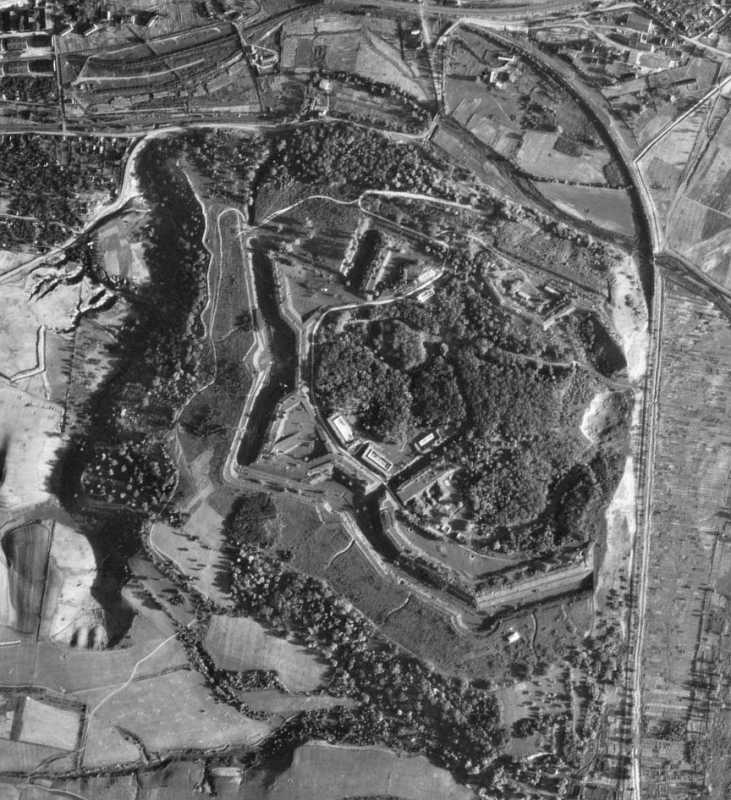
\includegraphics[width=\textwidth]{chast-lys-gory/zazver/aero.jpg}

\textit{Лысогорский форт на аэрофотоснимке 1943 года.}
\end{center}

Жертв тут же и хоронили, покуда хватало места. В 1910 году киевский полицмейстер просил власти выделить больше земли под могилы – и таки отвели особое кладбище на Старонаводницкой, часть Зверинецкого кладбища. В казну взыскивалась с родственников убиенных плата за казнь, 12 рублей.

Где именно на Лысой горе казнили? На плане Виккерса 1923 года, обозначены «8 виселиц» западнее места впадения речушки Бусловки в Лыбедь, по правому берегу последней (где она образовывала проточное озерцо – Бусловский пруд, некогда на нем была лаврская мельница), под склоном Лысой горы. На правом берегу Бусловского пруда была Лысая гора, на левом, между двумя параллельными железнодорожными ветками – Бусловский сад, бывший там и в 1940-х. Что до Бусловки, она течет сейчас в коллекторе вдоль улицы Киквидзе, к северу от Лысой горы.

Значит, место казней – к юго западу нынешнего перекрестка Саперно-Слободской и Киквидзе, на склоне Лысой горы примерно под прежней вышкой-глушилкой, ныне вроде ретранслятором цифрового телевидения.

В советское время, да и ныне в музее «Косой капонир» показывали черную карету, в которой приговоренных к смерти возили из Косого капонира на Лысую гору. Карета была запряжена одной лошадью, маршруты менялись, чтобы усложнить возможность напасть на карету и спасти заключенного.

На соседнем холме Зверинца, над Выдубичами, был Зверинецкий форт\footnote{Его остатки мы показали в фильме «Киевская амплитуда: Зверинецкий форт».} – склад боеприпасов. Это там, а не на Лыске, в 1918 году там произошли взрывы и пожар.

И вот после этого местом артиллерийских складов и стал Лысогорский форт. Закончилась гражданка, форт продолжал быть военным объектом – на стенах потерн\footnote{Пот\'ерна – подземный коридор в крепости.} осталось множество надписей, выцарапанных часовыми на крепких дореволюционных кирпичах с клеймами «ЭиЛ». Потерны, пробившие насквозь земляные валы, остались поныне – некоторые впрочем уже завалены с одного из входов. А валы заросли сверху деревьями.

% граффити часовых, вроде «Охранял пост мая 11, 1921. кур. г. обо. у м.в.о. сд. – Г. Я. Русанов».

До Великой Отечественной войны в форте хранили взрывчатые вещества. Территорию обнесли забором с колючей электрифицированной проволокой, поставили башни с охраной, завели овчарок. Когда немцы подступали к Киеву, наши эшелонами вывезли взрывчатку. Благо, железная дорога находилась рядом, под горой. Затем на горе заняли оборону наши войска.

После войны, на Девич-горе размещались артиллерийские склады, и для их обслуживания создали военную часть около озера Глинка\footnote{Озеро рядом с Лыбедской площадью, образовалось в карьере добычи глины.}. Там же был лагерь пленных немцев, работавших на кирпичном заводе и возводивших мост-путепровод через Лыбедь, между бульваром Дружбы Народов и Московской площадью. Боеприпасы на Лыске хранились в потернах, а подвозились и отвозились через железнодорожную ветку, что отходила вдоль склона к современному цементному заводу.

В 1970-х склады решили упразднить – мол, опасно. Хотя город уже давно подобрался к горе. Построили пожарную часть, чтобы временно хоть как-то усилить безопасность. К 1976 году снаряды вывезли, а охрану сняли. Жители с окрестностей начали растаскивать крепость на кирпичи. Гора быстро пришла в запустение – впрочем, она и была такой, никто там годами ничего не трогал, пока Лысую охраняли.

Помню, в начале 80-х, когда я был очень мал, меня повел на Лыску отец, показывал многовековой дуб у южной части форта. Наверное, только хоровод людей, взявшихся за руки, мог бы обхватить этот могучий ствол. Я забрался на развилку дуба, помню на ощупь его выпуклую, древнюю кору.

Росли там и другие, не менее древние дубы. Позже кто-то пытался их сжечь. Частично это удалось. Ныне на Девич-горе уцелело несколько дубов возрастом около пяти столетий, а то и больше, в разной степени сохранности.
 
 %Уцелевший поныне дуб, именуемый в народе «дубом-Ведуном» – жалкое подобие виденных мною дубов. Те были раза в четыре, а то и пять шире!

В 1982 году местность Лысой горы отвели под «природ\-но-ландшафтный парк» в честь 1500-летия Киева. Немного расчистили потерны, и потом дело остановилось.

Пока люди посещали заброшенную Девич-гору гостями, а не хозяевами, тут расцвела природа, можно было встретить краснокнижные растения и живность. Сейчас на ней постоянно происходит движение – по дорогам ездят машины, играет музыка любителей шашлыков, гудят экскурсии разного толка – от фортификационного до эзотерического, собираются неоязычники. 

Совершим небольшую прогулку. Снимки 30 апреля 2006 года сделаны моим отцом Владимиром Семилетовым и дедом Павлом Семилетовым. Остальные – мною в 2011-2016.

%Когда я был на Лыске в последний раз, кажется в 2009 году, летом, она представляла собой тихий, тенистый склон под огромными деревьями, местами поваленными. По склону идет утоптанная дорога, от нее в крутые яры спускаются тропы. У подножия есть заболоченное озеро, его называют «Лукрец», но тот ли этот старинный Лукрец из земельных документов? Наверху, после мрачной и комариной дороги – зелень, душистое разнотравье, полное гула пчел и шмелей. 


\begin{center}
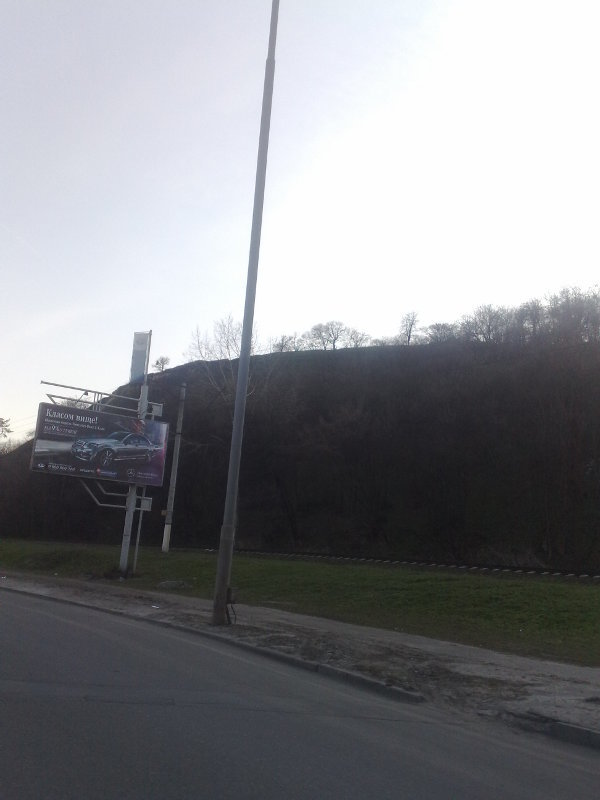
\includegraphics[width=0.91\textwidth]{chast-lys-gory/zazver/devich-gora-01.jpg}

\textit{2011. Вид на Лыску, ее восточный склон, со стороны шоссе.}
\end{center}

\newpage

\begin{center}
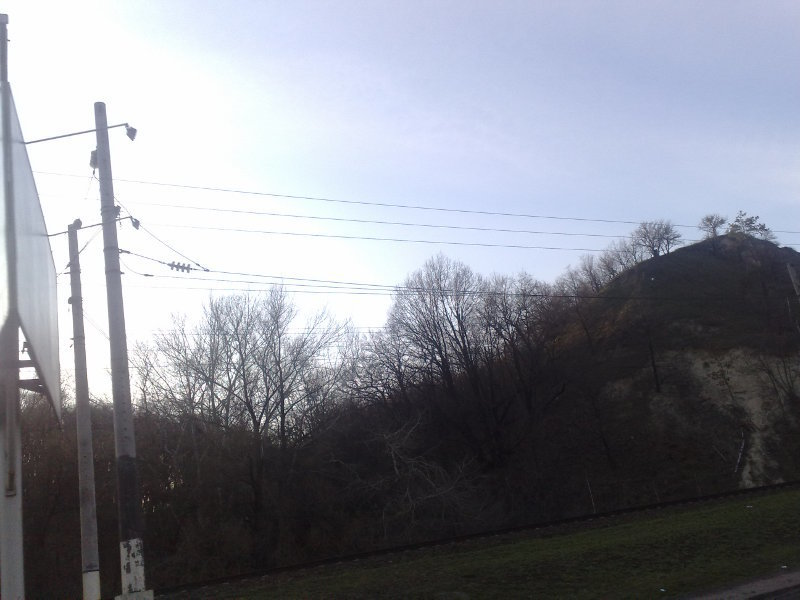
\includegraphics[width=0.93\textwidth]{chast-lys-gory/zazver/devich-gora-02.jpg}

\textit{2011. Чуть дальше. Тут меж двух отрогов горы, в удолье начинается восходящая к вершине дорога. Отрог справа ооочень высокий. По его угловой кромке есть узкая тропа.}
\end{center}

\begin{center}
\includegraphics[width=0.93\textwidth]{chast-lys-gory/zazver/\myimgprefix IMG_20160515_142758.jpg}

\textit{2016. Дорога в удолье.}
\end{center}

\newpage
\vspace*{\fill}
\begin{center}
\includegraphics[width=\textwidth]{chast-lys-gory/zazver/\myimgprefix IMG_20160515_143346.jpg}

\textit{2016. В сторону, на южный отрог, отходит крутая тропа. Вид с отрога, сверху.}
\end{center}
\vspace*{\fill}

\newpage
\vspace*{\fill}
\begin{center}
\includegraphics[width=\textwidth]{chast-lys-gory/zazver/\myimgprefix IMG_20160515_144610.jpg}

\textit{2016. Через гору идут спрямленные человеком овраги.}
\end{center}
\vspace*{\fill}

\newpage
\vspace*{\fill}
\begin{center}
\includegraphics[width=\textwidth]{chast-lys-gory/zazver/\myimgprefix IMG_20160515_145252.jpg}
\end{center}

\begin{center}
\includegraphics[width=\textwidth]{chast-lys-gory/zazver/\myimgprefix IMG_20160515_145443.jpg}

\textit{2016. Четвертая потерна с обеих сторон.}
\end{center}
\vspace*{\fill}
\newpage
\vspace*{\fill}

\begin{center}
\includegraphics[width=\textwidth]{chast-lys-gory/zazver/\myimgprefix IMG_20160515_150531.jpg}

\textit{2016. Другая потерна.}
\end{center}
\vspace*{\fill}

\newpage
\vspace*{\fill}
\begin{center}
\includegraphics[width=\textwidth]{chast-lys-gory/zazver/\myimgprefix IMG_20160515_150636.jpg}

\end{center}

\begin{center}
\includegraphics[width=\textwidth]{chast-lys-gory/zazver/\myimgprefix IMG_20160515_150632.jpg}

\textit{2016. Надписи у входов.}
\end{center}
\vspace*{\fill}
\newpage

\begin{center}
\includegraphics[width=\textwidth]{chast-lys-gory/zazver/\myimgprefix IMG_20160515_153612.jpg}

\textit{2016. Межовражие.}
\end{center}

\begin{center}
\includegraphics[width=\textwidth]{chast-lys-gory/zazver/\myimgprefix IMG_20160515_154023.jpg}

\textit{2016. Внутренние дороги форта.}
\end{center}

\newpage
\vspace*{\fill}
\begin{center}
\includegraphics[width=\textwidth]{chast-lys-gory/zazver/\myimgprefix IMG_20160515_154202.jpg}

\textit{2016. Почти там же, но в другую сторону.}
\end{center}
\vspace*{\fill}
\newpage


\begin{center}
\includegraphics[width=0.96\textwidth]{chast-lys-gory/zazver/\myimgprefix IMG_20160515_155020.jpg}

\textit{2016. Вид с северного отрога на юг, в сторону Корчеватого.}
\end{center}


\begin{center}
\includegraphics[width=0.96\textwidth]{chast-lys-gory/zazver/\myimgprefix IMG_20160515_155010.jpg}

\textit{2016. Вид чуть левее, впереди полосатые трубы пятой ТЭЦ.}
\end{center}


\newpage
\vspace*{\fill}

\begin{center}
\includegraphics[width=\textwidth]{chast-lys-gory/zazver/\myimgprefix IMG_20160515_155140.jpg}

\textit{2016. Вид на север, впереди слева – холм Зверинца, справа – промзона Теличка.}
\end{center}
\vspace*{\fill}

\newpage
\vspace*{\fill}
\begin{center}
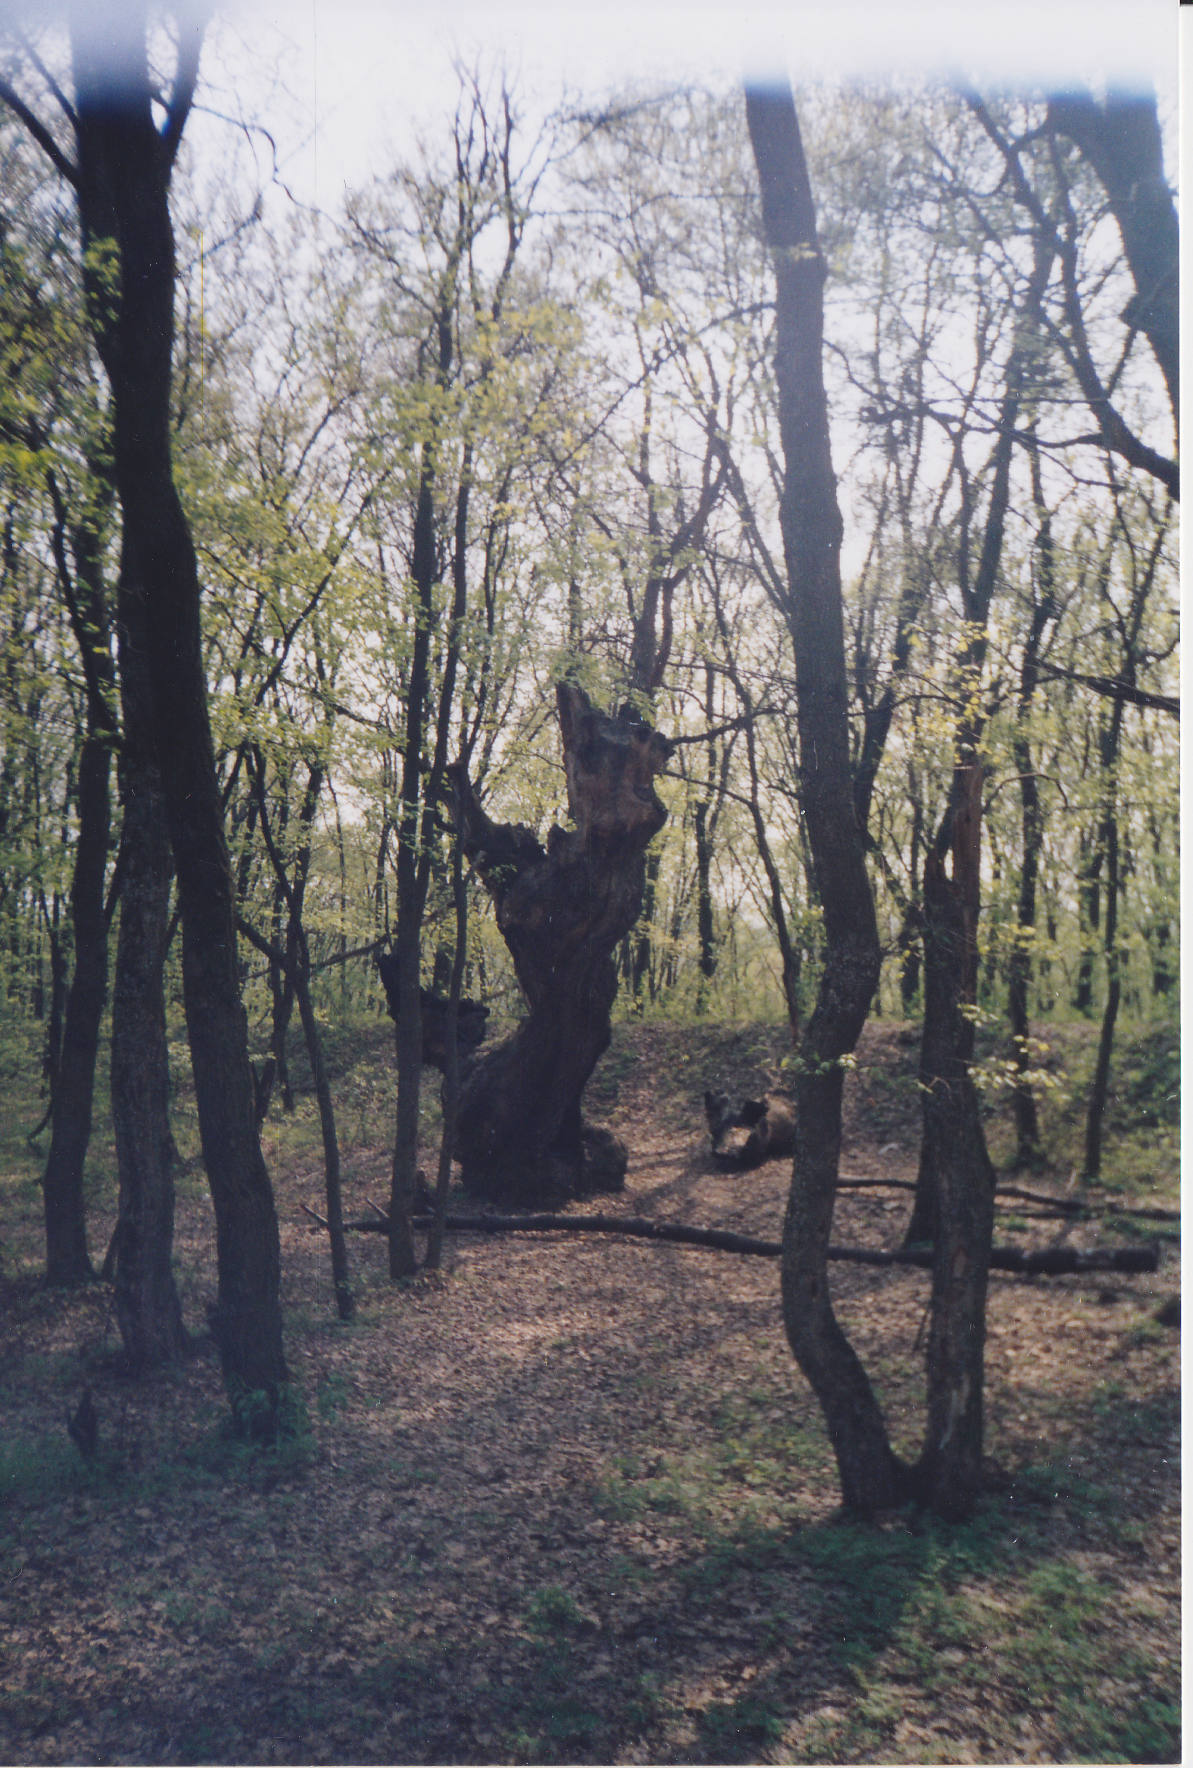
\includegraphics[width=\textwidth]{chast-lys-gory/zazver/stardub.jpg}

\textit{Апрель 2006. Остатки древнего дуба.}
\end{center}
\vspace*{\fill}
\newpage
\vspace*{\fill}
\begin{center}
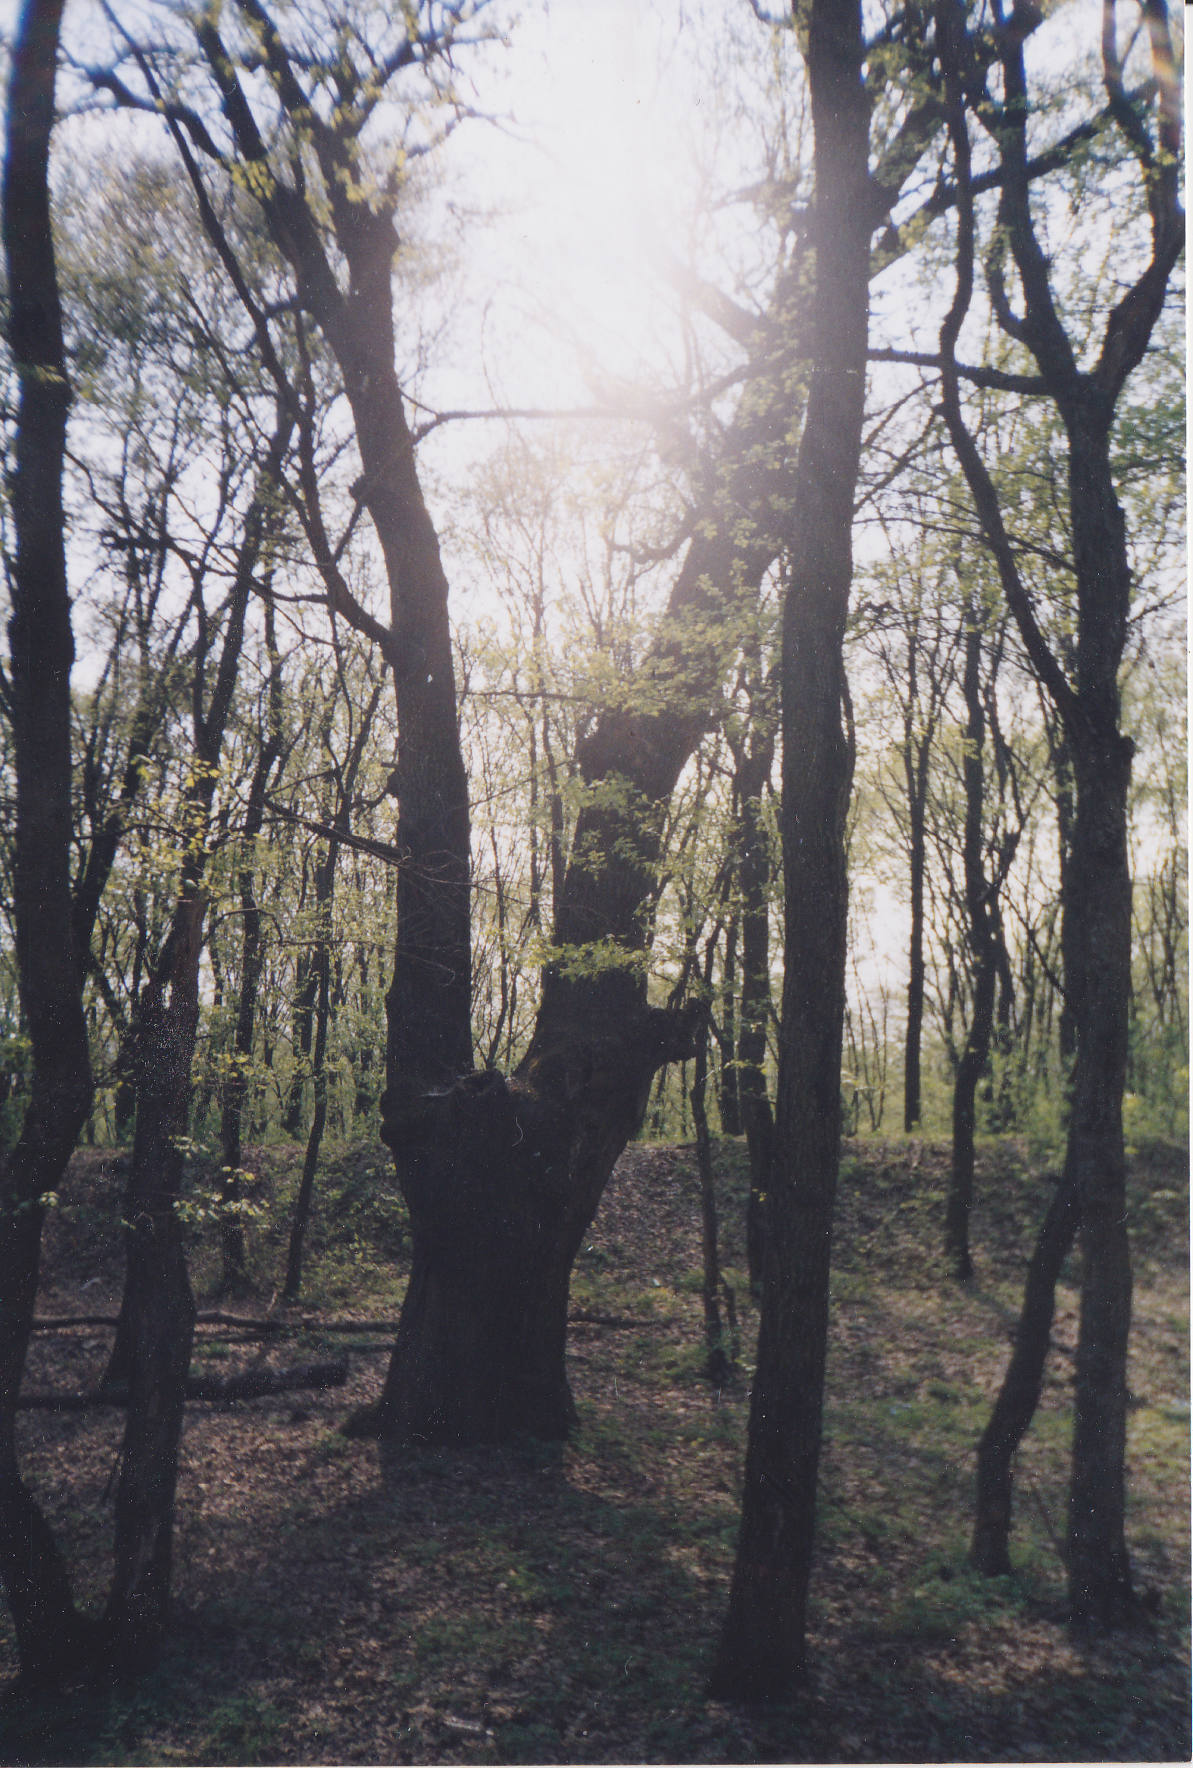
\includegraphics[width=\textwidth]{chast-lys-gory/zazver/stardub02.jpg}

\textit{Апрель 2006. Древний дуб.}
\end{center}
\vspace*{\fill}

\newpage
\vspace*{\fill}

\begin{center}
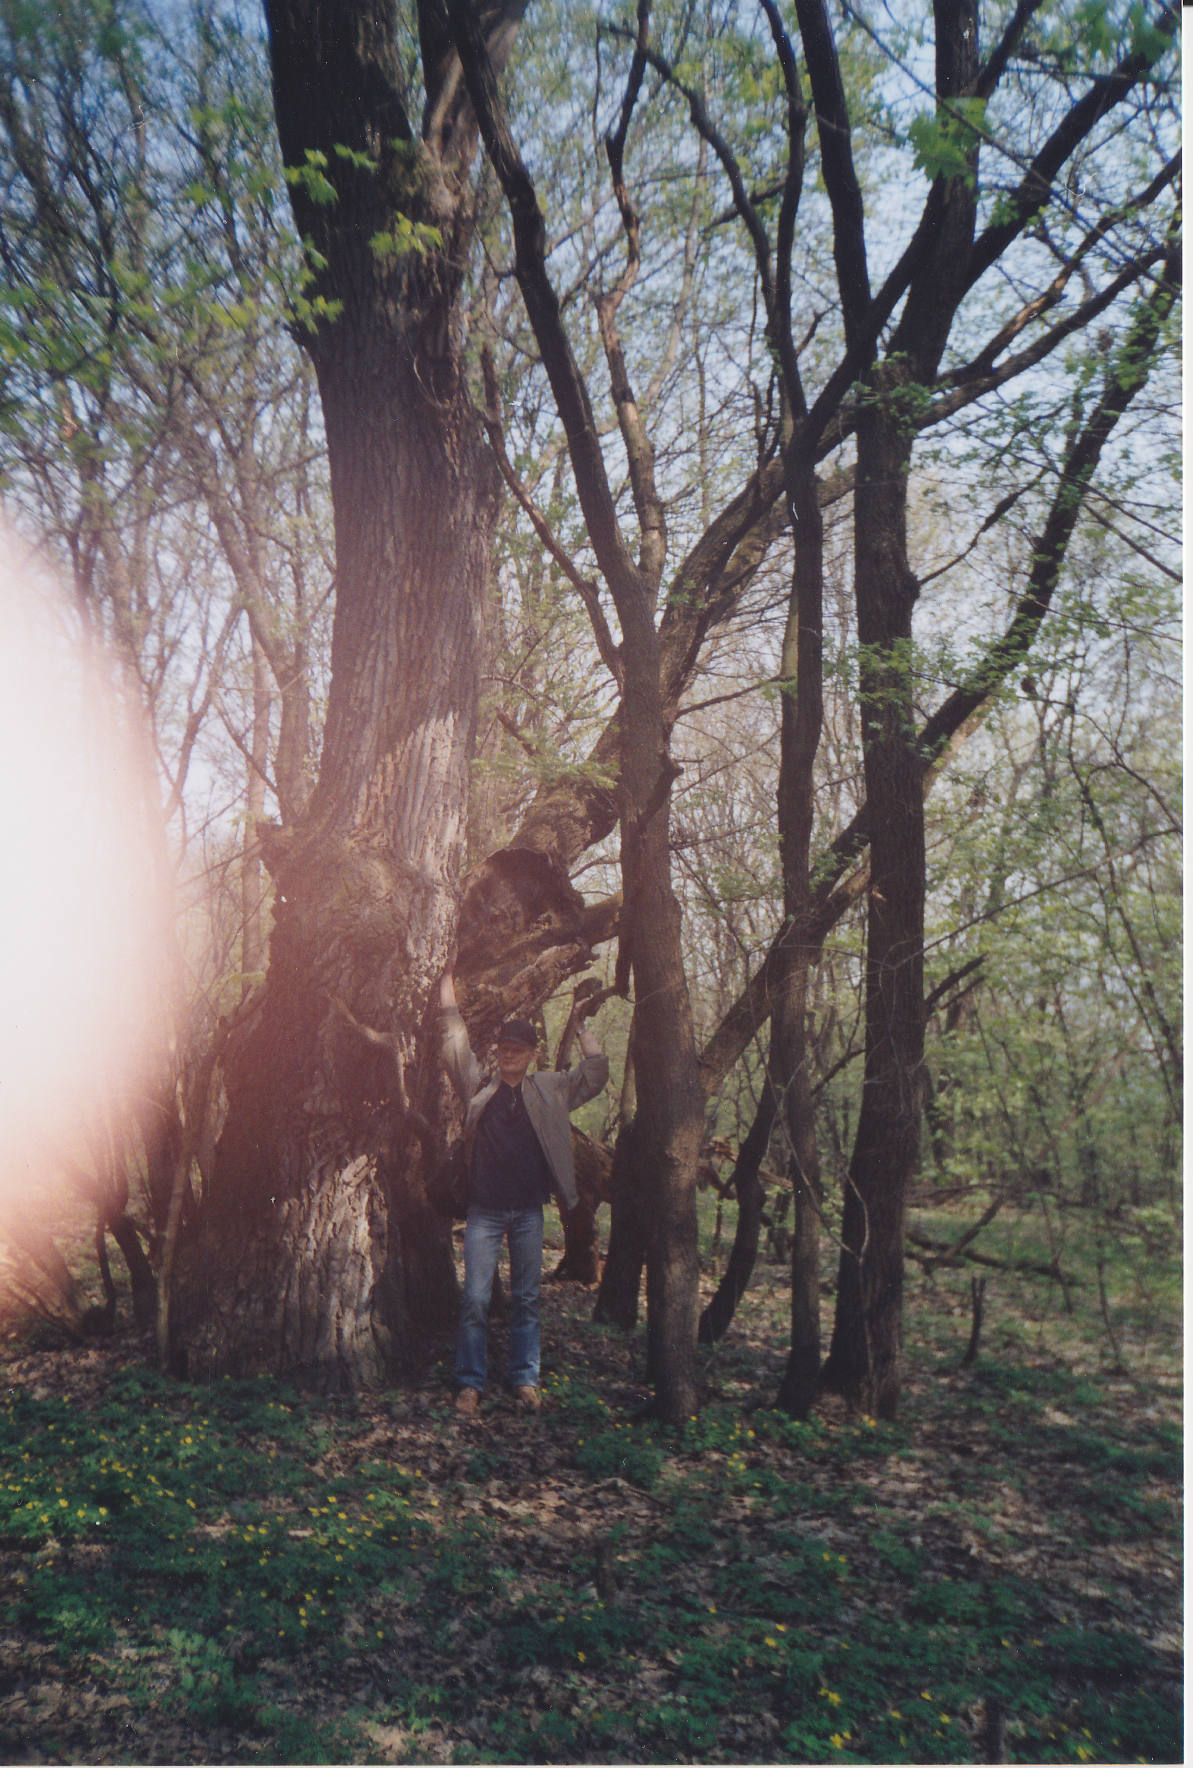
\includegraphics[width=\textwidth]{chast-lys-gory/zazver/stardub03.jpg}

\textit{Апрель 2006. Мой отец возле другого древнего дуба.}
\end{center}

\vspace*{\fill}
\newpage

\newpage

\begin{center}
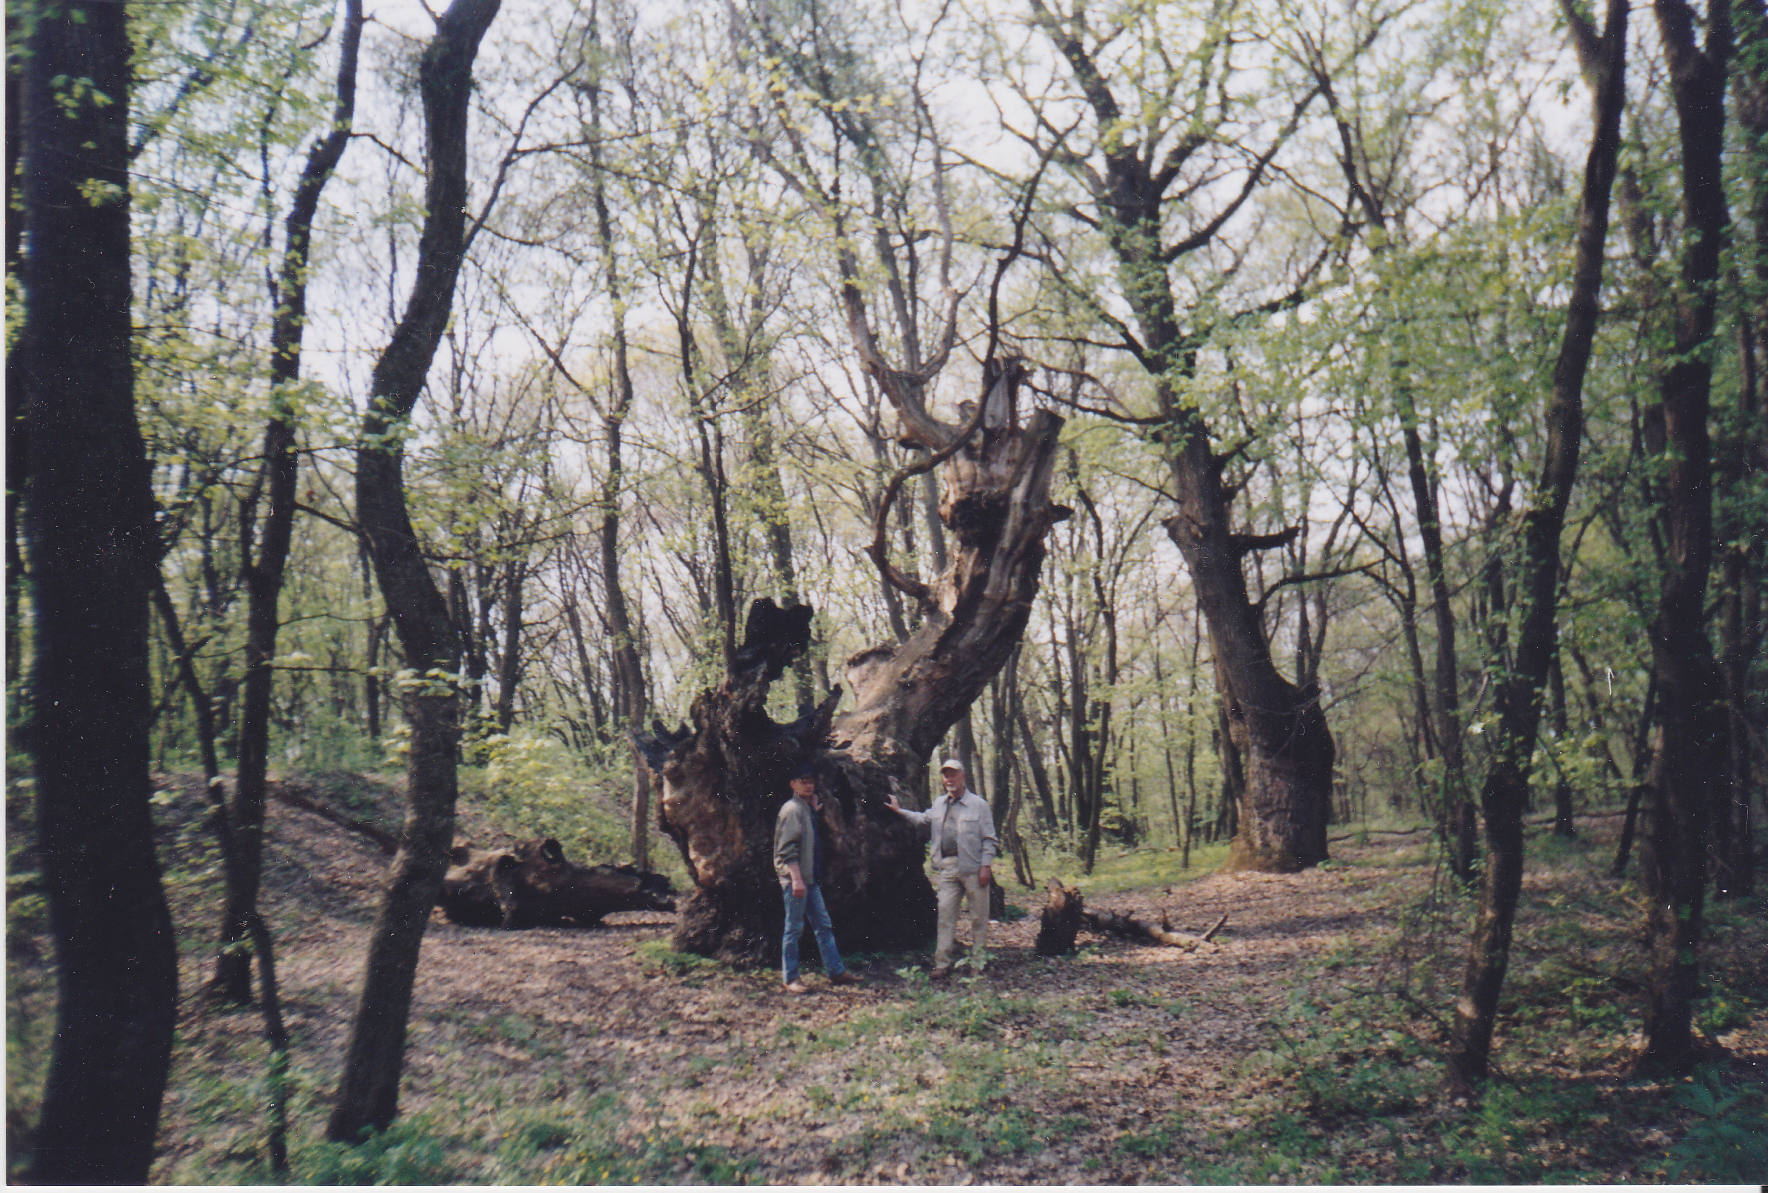
\includegraphics[width=\textwidth]{chast-lys-gory/zazver/stardub04.jpg}

\textit{Апрель 2006. Старейший дуб в Киеве. Рядом стоят Владимир и Павел Семилетовы.}
\end{center}

\vspace*{\fill}  

Немного об окрестностях Лысой горы. 

Северный её склон омывается Лыбедью. Приняв в коллекторе последний левый приток – речку Бусловку, Лыбедь выходит из бетонного подземелья на поверхность\footnote{50°23′58.6″N 30°33′13.3″E} за эстакадой пересечения улиц Киквидзе и Саперно-Слободской, чуть поодаль от дороги, идущей наверх Лысой горы.

Открытое русло вдоль подножия склона – спрямлено, правый берег его составляет склон Лысой горы, на левом – свалка и гаражный кооператив, у границы коего, около железнодорожной станции «Выдубичи-Трипольские», еще в первой половине 20 века было озеро на лугу, и вода прорывается там наружу поныне.

Близ Девич-горы Лыбедь наиболее полноводна, ибо это – низовье течения реки, она уже вобрала в себя все многочисленные притоки, так же, как и она сама, заточенные человеком в коллекторы. Желтоватая вода бурлит и несется потоком шириной с улицу.

\newpage

\begin{center}
\includegraphics[width=0.93\textwidth]{chast-lys-gory/zazver/\myimgprefix IMG_4439.jpg}

\textit{26 декабря 2015. Вид с Лысой горы в долину Лыбеди. Напротив – Бусова гора.}
\end{center}


\begin{center}
\includegraphics[width=0.93\textwidth]{chast-lys-gory/zazver/\myimgprefix IMG_4438.jpg}

\textit{26 декабря 2015. Вышла Лыбедь из коллектора. Вид на юго-восток. Справа – гора, слева – свалка вдоль гаражного кооператива.}
\end{center}

\newpage


\begin{center}
\includegraphics[width=0.98\textwidth]{chast-lys-gory/zazver/\myimgprefix IMG_4425.jpg}

\textit{26 декабря 2015. Там же.}
\end{center}


\begin{center}
\includegraphics[width=0.98\textwidth]{chast-lys-gory/zazver/\myimgprefix IMG_4444.jpg}

\textit{26 декабря 2015. Ближе к Столичному шоссе. Вид на северо-запад.}
\end{center}

\newpage
\vspace*{\fill}
\begin{center}
\includegraphics[width=\textwidth]{chast-lys-gory/zazver/\myimgprefix IMG_4441.jpg}

\textit{26 декабря 2015. Вид на юго-запад. Берега реки усеяны мусором, приплывшем со всего города.}
\end{center}
\vspace*{\fill}
\newpage

\begin{center}
\includegraphics[width=0.96\textwidth]{chast-lys-gory/zazver/\myimgprefix IMG_4445.jpg}

\textit{26 декабря 2015. Ближе к Столичному шоссе, вид на юго-восток.}
\end{center}


\begin{center}
\includegraphics[width=0.96\textwidth]{chast-lys-gory/zazver/\myimgprefix IMG_4448.jpg}

\textit{26 декабря 2015. Лыбедь в пересечении с железнодорожным мостом перед Столичным шоссе.}
\end{center}

\newpage

\begin{center}
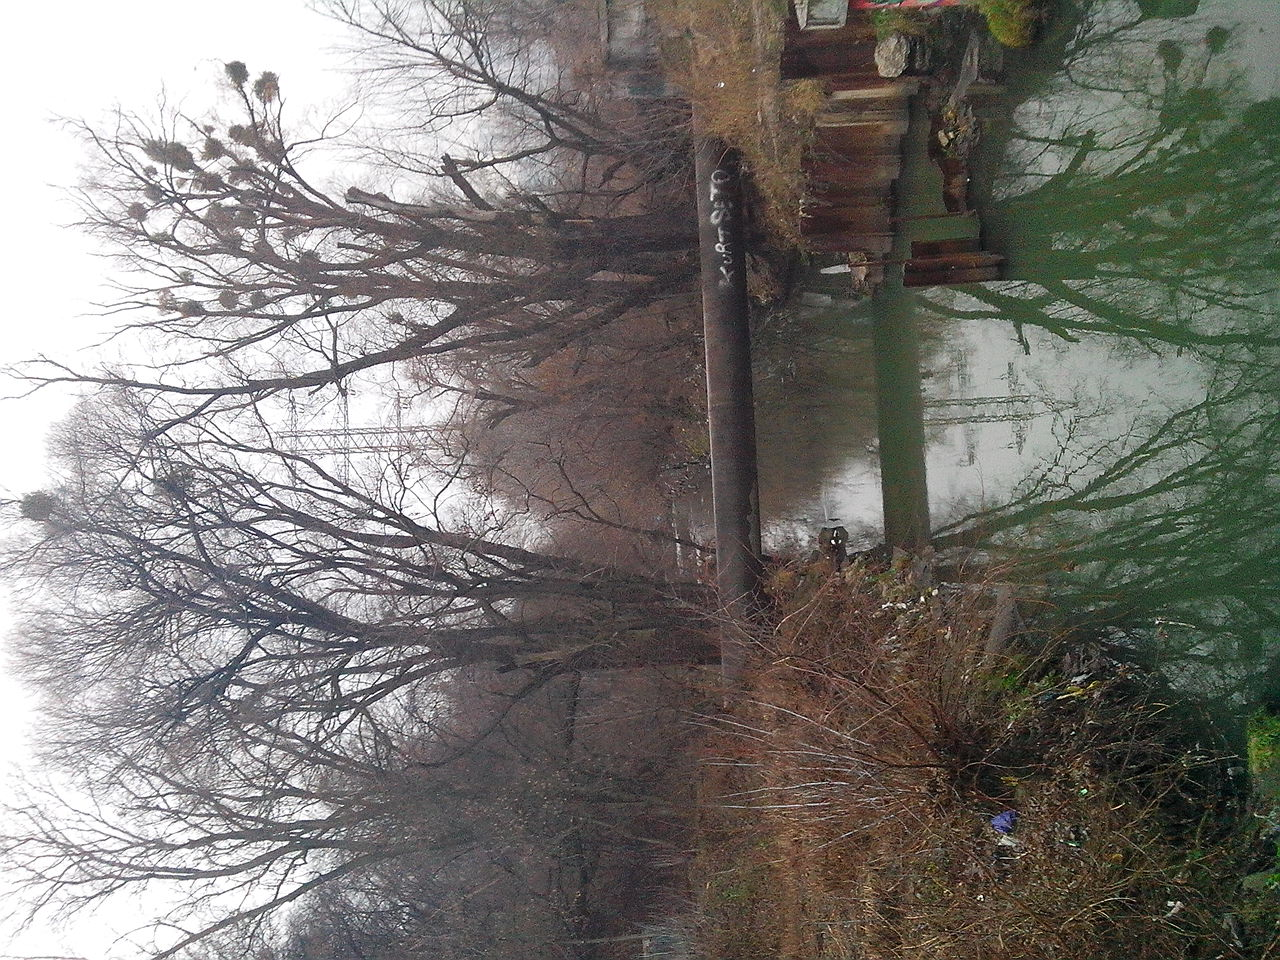
\includegraphics[width=\textwidth]{chast-lys-gory/zazver/IMG_20151226_150617.jpg}

\textit{26 декабря 2015. Вид с железнодорожного моста на северо-запад. Лысая гора – слева.}
\end{center}

У Столичного шоссе, Лыбедь сворачивает на юго-восток еще более резко, по искусственному каналу вдоль улицы Промышленной, и впадает в Днепр на широте Багриновой горы. Прежде было иначе. На местность повлияло много причин, в том числе строительство Дарницкого железнодорожного моста. Я без точной привязки ко времени попытаюсь проследить смещение устья Лыбеди.

В середине 19 века широкий рукав Днепра примыкал почти к Лысой горе, там же впадала Лыбедь. От конца улицы Тимирязевской до самой Мышеловки по Днепру лежало пять больших островов, образованных наносами, выброшенными Лыбедью в Днепр. Эти острова носили общее имя – Галерный.

У подножия Лысой горы, напротив «главной» дороги по восточному ея склону, на Днепре была пристань.

Строительство железнодорожного Дарницкого моста и другие причины привели к изменениям местности. Большой рукав Днепра вдоль восточного склона Лысой горы, стал \'уже, получил название Лысогорского. Часть островов между Лысой горой и Осокорками объединились в большой, разделенный проливом, остров Галерный.

Ближе к концу 19 века верховья Лысогорского рукава обмелели и обратились в сушу. Низовья рукава образовали известный поныне залив Старик\footnote{Был еще один Старик между Выдубичами, железной дорогой, Днепром и Теличкой – поначалу рукав Днепра, потом озеро, застроенное ныне промзоной.} (на картах его ошибочно называют «Галерный»), прежде Чернечий. 

Так русло Днепра сместилось на восток. В ту же сторону потекла Лыбедь от нынешнего шоссе, по теперешней промзоне Теличке, а устье ее было немного выше Южного моста. Итак, Лыбедь сохранила прежнее направление, но русло ее продлилось по суше прежних островов, припаявшихся к материку.

%В первой половине 20 века, по ряду причин это устье закрылось, и русло пошло на юг, примерно между Днепром и шоссе – не как теперь, наискосок, а параллельно шоссе. Дальше, пробежав мимо теперешней ТЭЦ-5, Лыбедь впадала в залив у низовья Галерного острова.

В первой половине 20 века, по ряду причин это устье закрылось, и русло пошло на юг, примерно между Днепром и шоссе – не как теперь, наискосок, а параллельно шоссе. Дальше, пробежав мимо теперешней ТЭЦ-5, Лыбедь впадала в залив в полукилометре южнее нынешнего устья.

Сейчас, западнее сего прежнего устья Лыбеди, на широте Мышеловки, был и остается Ерик. Неверно писать «залив Ерик» или «озеро Ерик». Само слово «ерик» значит «старица» или «залив». На современных картах также ошибочно показан залив Николайчик как западная часть Ерика. Однако настоящий Николайчик был устьем Лыбеди восточнее Ерика. Николайчик впадал в Днепр с севера в том месте, где с запада было устье залива Старика (Чернечего), обозначаемого ныне как Галерный.

Около Галерного острова, напротив Мышеловки, в Днепр вливались воды ручьев, текущих из Голосеево\footnote{По другую сторону Голосеевского холма тоже бежит, через пруды, ручей Ореховатка (назван так по хутору Ореховому), приток Лыбеди.} и Китаево – наиболее значительный ручей называется Голосеевским, на нем поныне есть несколько больших прудов. Низовья этих ручьев взяты в коллектор, соединяются около Столичного шоссе и общим коллектором идут в залив Старик (Галерный).


\begin{center}
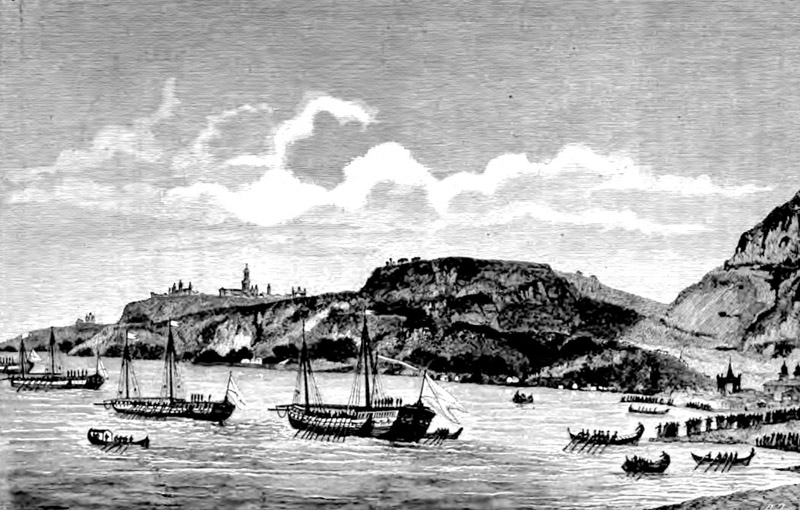
\includegraphics[width=\textwidth]{chast-lys-gory/zazver/otplytie-ekateriny-iz-kieva-1787.jpg}

\textit{Императорские галеры, отплывающие из Киева. 1787 год. Гравюра по рисунку художника Хатфильда.}
\end{center}

Современный, обозначенный на картах остров Галерный – только южная часть прежнего Галерного. Около него, с весны 1786 по весну 1787, стояли на причале галеры, сделанные под руководством англичанина Сэмюэла Бентама в Смоленске\footnote{Дело было поручено еще в 1784 году вице-адмиралу Пущину.} и пригнанные сюда к посещению Киева Екатериной II для путешествия ее в Херсон через Екатеринослав. Потемкинский блеск. 3 мая флотилия, насчитывающая 13 галер в римском стиле, и 13 поменьше, отплыла из Киева, от Подола.

Флотилию Екатерины II на диковинном червеобразном судне, «вермикуларе», догонял и сам подполковник Сэмюел Бентам. Очевидец, Франсиско де Миранда описывает это в «Путешествии по Российской империи», главе про Киев (даты по старому стилю)\cite{demiranda}:

\begin{quotation}
30 апреля. Рано утром заехал комендант, сообщивший об удивительном корабле Бентама и о том, что последний собирается навестить меня. Мы отправились вместе повидать его и его судно. Обратил внимание на комендантскую упряжку: отменные лошади и какие ухоженные! Приехали к Дашкову, где находился Бентам, исхудавший и сильно ослабленный лихорадкой.

Оттуда заехали к фельдмаршалу, предложив ему взглянуть на вышеупомянутое сооружение. Он согласился, мы уселись в кареты и спустились к пристани. Там поднялись на это судно, каковое имеет следующие особенности: оно состоит из шести отдельных корпусов, сочлененных так, что корабль способен изгибаться наподобие червяка, и это самое поразительное сооружение, какое только можно себе представить, в то же время как нельзя более подходящее для плавания в подобных местах; ибо его осадка не превышает семи дюймов, и оно движется и поворачивает куда угодно, словно змея. Длина его – 252 фута, ширина – 16, а высота бортов, считая от киля, не более 12 футов, так что на нем со всеми удобствами может разместиться изрядное количество людей\footnote{Длина 77 метров, ширина 5, высота бортов 3,7.}. Судно оснащено 120 веслами и движется со скоростью от 10 до 12 верст в час\footnote{10-13 километров в час.}. Отплыв от пристани, мы попробовали управлять им, и было любопытно наблюдать, как это червеобразное – так именует свое судно его создатель – изгибалось и поворачивало то в одну, то в другую сторону, совсем как угорь. Бентам сообщил нам, что все от начала до конца придумано им самим, и что корабль обошелся ему в 9 тысяч рублей, кои он выложил из собственного кармана. Мы очень сожалели, что он не поспел к отплытию императрицы, ибо его судно по скорости хода и надежности превосходит галеры, на которых отбыла Ее Величество, да и своей необычностью наверняка пришлось бы ей по вкусу.
\end{quotation}

Предприимчивый механик, корабел Сэмюэл Бентам – брат английского философа-утилитариста Джереми Бентама – был приглашен в Россию Потемкиным в 1780 году как специалист по кораблестроению, пивоварению, и в качестве приказчика имений Потемкина в Белоруссии, в Кричеве. Бентам покорил князя своим экипажем-амфибией, что из колесного легко превращался в лодку.

Причудливый, извивающийся корабль-червь происходил из причудливого мировоззрения братьев Бентамов. Бентам-философ предлагал устроение паноптиконов – круглых, будто головы сыра, зданий для надзора для содержащимися там людьми. Это могли быть тюрьмы, школы, сумасшедшие дома, больницы. Паноптикон управляется с башни, откуда надзиратель следит за «подопечными», и через особые трубы раздает приказы в нужные ячейки, либо подслушивает чужие разговоры. Отапливать камеры Бентам предлагал через другие трубы, вроде дымоходных, подавая по ним огнем нагретый воздух.

В Англии проект Паноптикона не прокатил, в Кричиве его собирались воплотить в жизнь, но Крымская война сорвала задумку братьев. К слову, Сэмюэл в бытность управляющим имением Потемкина сделал несколько кораблей-червей для перевозки лесоматериалов и провианта.

На основе чертежей Паноптикона, в 1807-09 годах в Петербурге Сэмюэл построил школу-фабрику кораблестроителей, чтобы те учились и на месте сами производили необходимое навигационные приборы, шили морскую форму и так далее. Здание стояло на речке Охте и сгорело в 1818 году. За подробностями отсылаю вас к работе Филипа Стэдмена «Паноптикон Сэмюэла Бентама»\cite{panoptikon}, да есть и другие публикации, вытаскивающие из архивного мрака странные дела прошлого.

Джереми был идейным вдохновителем, Сэмюэл – более воплотителем. Джереми рвался к законотворчеству, в Англии и России, где его философские труды печатались в переводе. Имел вес! Однако с Александром I столковаться не удалось. Вскоре впрочем царь с Аракчеевым принялись муштровать Русь военными поселениями.

Незадолго до смерти в 1832 году Джереми Бентам завещал сделать из себя чучело и показывать в коробе с дверкой. Его по сей день иногда показывают в Лондоне. Что до Сэмюэла, по возвращении из России он построил первый стальной мост через Темзу (Vauxhall Bridge, нынешний Vauxhall Bridge – другой, новее, заменивший прежний), затем переселился во Францию, откуда сбежал обратно в Англию, ибо нарушил водную систему местности орошением своих полей, и соседние землевладельцы подали на него в суд.

Но вернемся к нашей, киевской водной системе. 

Современный залив Старик около острова Водников – ниже истинного Старика. Я же упорно буду называть Стариком то, что теперь подписывают как залив Галерный.

Есть на картах еще, я проследил с 1902 года, слово «покал», значение коего не знаю. На плане 1902 года, южнее урочища Нижняя Теличка и дровяных складов, обозначена некая область с подписью «Остров Покал Галерный». Примерно там же, то бишь между Лысой горой и тогдашним руслом Лыбеди, проходящему параллельно восточному склону горы в некотором отдалении от него, на немецких картах 1940-х отмечено урочище Pokal (что кстати в переводе с немецкого значит «чашка», сравните с нашим «бокалом»). Затем уже на советских картах написано: «Покол».

Зная последовательность появлений сего названия на картах, можем предположить, что его отчекрыжили от острова Галерного, имевшего полное название «Покол Галерный». Современный «Покал» это одна из уцелевших частей Галерного острова. Кстати, низовье Лыбеди долгое время использовалось для сброса неочищенных сточных вод с Верхнего города и Подола.

К востоку от Лыски есть охладительный канал ТЭЦ-5, где каменистое дно, дикое течение и вода тёплая, будто в ванной. Я там однажды плавал.

Напротив Лыски, на север, лежат два холма – условно говоря Зверинецкий, и Бусова или Буслова гора, переходящая в Черную гору, что ближе к озеру Глинка и бульвару Дружбы Народов. Между Лысой и этими горами, в долине Лыбеди, проходит железная дорога и улица Сапёрно-Слободская, северная сторона которой называется Саперной слободкой. По улице, от Демиевки, в 1913 году проложили трамвайную линию до станции Киев-2 (Киев-Московский). Линию демонтировали в конце 1920-х.

Однако уже в тридцатые восстановили маршрут, идущий по нынешней Бастионной улице, который затем сворачивал от ее верха на Зверинескую и затем вниз, на Сапёрную слободку. До революции он, под номером 12, доходил лишь до – относительно современности – спуска Сиреневой аллеи в ботсаду. Конечно, маршрут давно снят!

Встречается мнение, что на Девич-горе находилась крепость сестры Кия, Хорива и Щека – Лыбеди. На это нет никаких указаний. Да, из списков летописей мы имеет смутные указания вроде:

\begin{quotation}
Сестра же их Лыбедь над рекою Лыбедью свои осады положиши, таможе и город на пригорку высоком согради от своего имени Лыбедь.\end{quotation}

Разве по этим строкам можно понять, о какой горе идет речь? Максим Берлинский в 1820 году писал про Лыбедь:

\begin{quotation}
В трех местах на холмах по левую сторону Лыбеди и на одной с противной стороны, по оставшемуся щебню видны следы жилых мест, но может быть они гораздо позднейших времен, нежели село Предславино\footnote{Известное по летописи село возле Лыбеди.}
\end{quotation}

По ходу русла есть множество гор – хотя бы у Протасова яра или в остатках Кадетской рощи по улице Уманской.

Если же в давнее время началом Лыбеди считались не истоки в Отрадном и на Кардачах, а ручей, известный сейчас как Скоморох, то местом обитания сестры Лыбеди могут быть и холмы над цирком, где сейчас улица Чкалова (Гончара, Маловладимирская) и Бульварно-Кудрявская (Воровского). Учитывая кучность гор, где жили братья, гору Лыбеди вероятнее искать ближе к родичам.

Хотя не следует сбрасывать со счетов экономические соображения. Например, в ближайшие к нам века на Лыбеди, близ нынешних вокзала и Московской площади, были переправы торговых дорог. Горы братьев – Киевица, Щекавица, Юрковица – именные, и являются высотами, ограничивающими взъезд во внутреннее пространство города через яры, с восточной стороны. Почему речка Лыбедь не может быть именной, от сестры Лыбеди? 

Каждый член семейства не просто сидел себе на горе или у реки, а брал с купцов пошлину за прохождение через «свою» дорогу. Братьям достались пути с востока, да идущие по Днепру, и вероятно северные, а сестре – не менее выгодный набор дорог через речку Лыбедь, подпоясывающую город с юга и запада.

Это приводит к еще одному вопросу – так ли, как нам говорит наука, невелик и первобытен был Киев во времена Кия, Хорива, Щека и Лыбеди, а также до них?
